\chapter{Survey}
\label{survey}

Surveys gather information through questions on a sample of people.
They can take many forms, including telephone surveys, face-to-face surveys, paper surveys, and online surveys.
Unlike other forms, online surveys benefit from being faster, cheaper, more accurate, and easy to get and analyze.

Online surveys often consist of open-ended and closed-ended questions that help analyze the studied topic.
They can also contain different questions based on participants' roles.
There are also dedicated applications to create and conduct online surveys that can set up different questions, separate them into individual groups or pages, make conditions to display them only to specific user roles, etc.

The first important task is defining the survey's goals and who to survey.
With that in mind, questions are created.
And in the end, the gathered data has to be analyzed.
It is often required to process and adjust the data before analyzing, especially the open-ended questions.
Therefore a human worker must go through these questions and take out the relevant data.

\section{Conducted Survey}

Even though this thesis focuses on developing a prototype mainly focused on children, also parents and teachers participated in it.
The game's future development counts on developing more features to include these user groups in the children's education.

Articles mentioned in the introduction also analyzed some use-cases of gamification in education or educational games.
These studies have been analyzed, and the conducted survey follows and considers their results. 

The primary purpose of the conducted survey for this thesis was to understand what some children, their parents, and teachers think and would make them motivated in a gamified game.

The survey recognizes three participant roles: a child, a parent, and a teacher.
Each role has a modified set of questions.

\subsection*{Questions asked only to children}

\begin{enumerate}
    \item What (non-educational) games do you usually play and why? What is your motivation for playing them? (Open-ended question.)
    \item Do you like receiving points as a reward for completing tasks? (Closed-ended question.)
    \item Do you like rankings in educational games? (Closed-ended question.)
    \item Would you like an advanced final task as a challenge? (Closed-ended question.)
    \item What is your primary motivation to play an educational game? (Open-ended question.)
\end{enumerate}

\subsection*{Questions asked to children, parents, and teachers}

\begin{enumerate}
    \item What aspects or mechanics are important in an educational game according to you? ((Closed-ended question with options: a game; a story; study materials; an explanation.)
    \item Do you (or your children/students) use any educational application or game? (Closed-ended question with options: Duolingo, Khan Academy, Minecraft, Scratch, other.)
    \item What experiences do you have with educational applications or games. What aspects do you like the most, what don't you like? (Open-ended question.)
    \item What would you appreciate most in an educational game? (Open-ended question.) 
\end{enumerate}

\subsection*{Questions asked only to parents and teachers}

\begin{enumerate}
    \item What is important to you? (Closed-ended question with options: progress monitoring; checking the results; ratings and comparison with other players; planning tasks for children to practice; an option to change child's settings.) 
\end{enumerate}

\section{Evaluation}

The~survey where children, parents, and teachers participated was held online using Google Forms.
An equivalent face-to-face survey was also done with children.
Both groups showed, on average, the~same results.

The~assumptions before doing the~survey were that at least 90 percent of respondents play non-educational games;
respondents (especially children) play some building games (such as Minecraft), children are mostly (at least 75 percent) competitive, and the~most crucial aspect is the~game itself, explanation, and a~story.

The~survey results pointed out that almost 22 percent of respondents do not play non-educational games.
Almost 18 percent of respondents (primarily children) play building games.
Respondents also chose to play casual games and shooting games in almost 14 percent of responses, puzzle or strategy games in nearly 12 percent of responses, board games, battle-royal-like games, and shooting games in about 7 percent.
The~results of which non-educational games people play are shown in figure~\ref{fig:survey:games}.

\begin{figure}
    \centering
    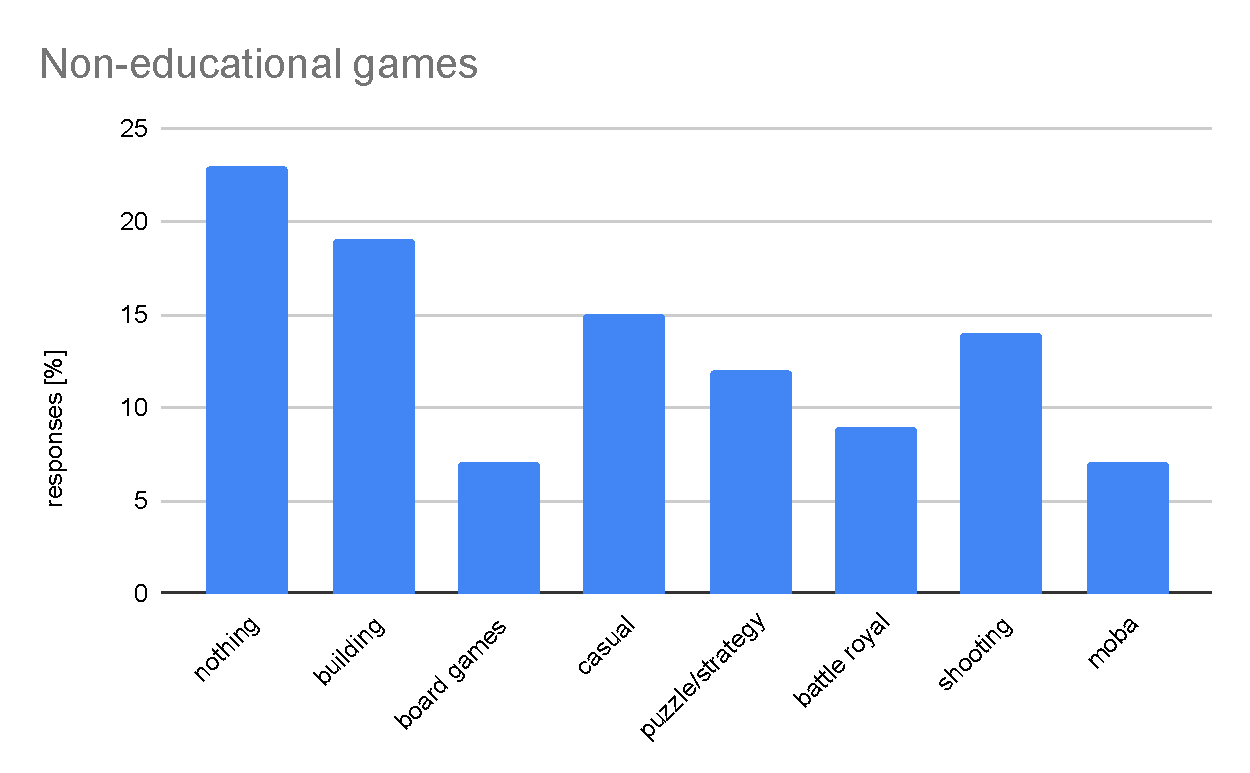
\includegraphics[width=1\linewidth]{assets/survey/non-educational-games.pdf}
    \caption{Played Non-educational Types of Games}
    \label{fig:survey:games}
\end{figure}

In a~matter of educational games people use, almost 60 percent of respondents use Duolingo~-- language learning educational game.
Almost 30 percent of respondents also selected Minecraft~-- a~game known for its building mechanics and an~option to program with unique blocks.
Almost 15 percent of respondents use Scratch~-- a~tool to do visual programming.
Other minor answers were, for example, Khan Academy and Kahoot with almost 7 percent.  

Focusing on children's answers, almost 80 percent like receiving some reward for completing tasks; nearly 75 percent like rating systems; and almost 80 percent of respondents would like the~last task to be a~challenge.

Questions about what aspects or mechanics are important in an~educational game showed exciting differences.
While children selected with the~same share a~game, a~story, and an~explanation, almost none selected study materials.
Parents and teachers selected a~story and an~explanation, while almost none chose a~game and study materials.
Interestingly, the~difference between children and parents or teachers is the~view on the~importance of the~game aspects.

The~results and initial assumptions contradict that most people play non-educational games; confirm that building games are the~most common kind of games children play; and show that children are~-- majority with almost 75 percent~-- competitive. 

The~conducted survey with the~addition of articles mentioned in the~introduction suggests that gamification in educational games might introduce valuable benefits.
In summary, children like to receive rewards in some form of points, want to compete and be rated, and like challenges.
All these factors underline the~motivational aspects found in mentioned studies,
as they help to increase the~attention span.

